\let\negmedspace\undefined
\let\negthickspace\undefined
\documentclass[journal]{IEEEtran}
\usepackage[a5paper, margin=10mm, onecolumn]{geometry}
\usepackage{tfrupee} 
\setlength{\headheight}{1cm} 
\setlength{\headsep}{0mm}     

\usepackage{gvv-book}
\usepackage{gvv}
\usepackage{cite}
\usepackage{amsmath,amssymb,amsfonts,amsthm}
\usepackage{algorithmic}
\usepackage{graphicx}
\usepackage{textcomp}
\usepackage{xcolor}
\usepackage{txfonts}
\usepackage{listings}
\usepackage{enumitem}
\usepackage{mathtools}
\usepackage{gensymb}
%\usepackage{wasysym}
\usepackage{comment}
\usepackage[breaklinks=true]{hyperref}
\usepackage{tkz-euclide} 
\usepackage{listings}
\def\inputGnumericTable{}                                 
\usepackage[latin1]{inputenc}                                
\usepackage{color}                                            
\usepackage{array}                                            
\usepackage{longtable}                                       
\usepackage{calc}                                             
\usepackage{multirow}                                         
\usepackage{hhline}                                           
\usepackage{ifthen}                                           
\usepackage{lscape}
\usepackage{circuitikz}
\tikzstyle{block} = [rectangle, draw, fill=blue!20, 
    text width=4em, text centered, rounded corners, minimum height=3em]
\tikzstyle{sum} = [draw, fill=blue!10, circle, minimum size=1cm, node distance=1.5cm]
\tikzstyle{input} = [coordinate]
\tikzstyle{output} = [coordinate]
\renewcommand{\thefigure}{\theenumi}
\renewcommand{\thetable}{\theenumi}
\setlength{\intextsep}{10pt} % Space between text and floats
\numberwithin{equation}{enumi}
\numberwithin{figure}{enumi}
\renewcommand{\thetable}{\theenumi}

\begin{document}

\bibliographystyle{IEEEtran}
\vspace{3cm}

\title{9.4.45}
\author{EE25BTECH11032 - Kartik Lahoti}
\maketitle

\subsection*{Question: } 

A motor boat whose speed is $18 \,km/h$ in still water takes $1$ hour more to go $24\,km$ upstream than to return downstream to the same spot. Find the speed of the stream.

\textbf{Solution}:\\

Let speed of boat be $v$ and of stream be $u$. 

Now, if $x-axis$ represents time $t$ for downstream and $y-axis$ represents time $t$ for upstream, 

\begin{align}
    \vec{n}^{\top}\vec{x} = c \label{eq_1}
\end{align}

where $c$ is distance $\brak{\text{Given }=24}$ and

\begin{align}
    \vec{n} = \myvec{1 & 1\\ 1 & -1}\myvec{v \\ u}
\end{align}

If Line \ref{eq_1} cuts $x-axis$ at $t_1$ and $y-axis$ at $t_2$, then 

Given,

\begin{align}
    t_1 = t_2 - 1
\end{align}

To solve, 

\begin{align}
    \myvec{v & u}\myvec{1&1\\1&-1}\myvec{t_2-1\\0} &= 24 \label{eq_4} \\
    \myvec{v & u}\myvec{1&1\\1&-1}\myvec{0\\t_2} &= 24  \label{eq_2}
\end{align}

From \ref{eq_2}
\begin{align}
    t_2 = \frac{24}{v-u} \label{eq_3}
\end{align}
Putting \ref{eq_3} in \ref{eq_4} , we get
\begin{align}
    u^2 + 48u - 324 = 0 \\
    \implies y = x^2 + 48x - 324 = 0 
\end{align}

which can be expressed as the conic

\begin{align}
    \vec{x}^{\top}\vec{V}\vec{x} + 2\vec{u}^{\top}\vec{x} + f = 0 \label{eq_5}\\ 
    \vec{V} = \myvec{1 & 0 \\ 0 & 0 } , \vec{u} = \myvec{24 \\ -\frac{1}{2}} , f = -324.
\end{align}

To find the roots of \ref{eq_5}, we find the points of intersection of the conic with the $x$-axis

\begin{align}
    \vec{x_i} + \vec{h} + k_i\vec{m} \\ 
    \vec{h} = \myvec{0\\0} , \vec{m} = \myvec{1\\0}
\end{align}
Using , 
\begin{align}
    k_i = \frac{1}{\vec{m}^{\top}\vec{V}\vec{m}}\brak{-\vec{m}^{\top}\brak{\vec{V}\vec{h}+\vec{u}} \pm \sqrt{\sbrak{\vec{m}^{\top}\brak{\vec{V}\vec{h}+\vec{u}}}^2-g\brak{\vec{h}}\brak{\vec{m}^{\top}\vec{V}\vec{m}}}}
\end{align}

\begin{align}
    k_i = \frac{1}{1}\brak{-24 \pm \sqrt{24^2 + 324}} \\ 
    \implies k_1 = 6 , k_2 = -54
\end{align}

Hence the points of intersection are 

\begin{align}
    \vec{h} + k\vec{m} = \myvec{6 \\ 0 } , \myvec{-54\\0}
\end{align}

Since $u$ cannot be negative , 
\begin{align}
    u = 6\,km/h
\end{align}

\begin{figure}[H]
    \centering
    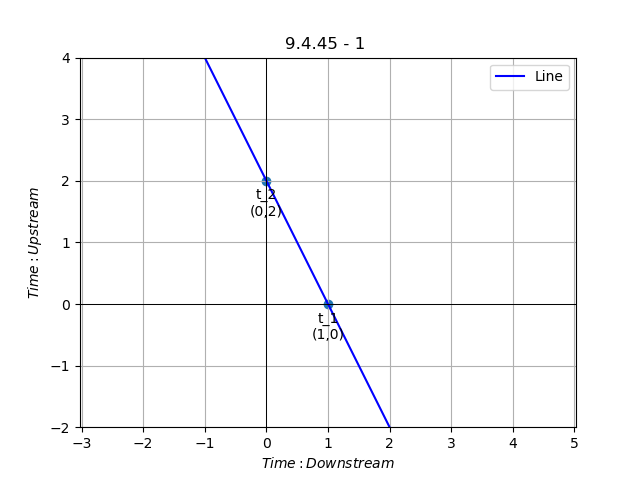
\includegraphics[width=0.5\columnwidth]{figs/graph1_1.png}
    \caption*{}
    \label{fig:placeholder}
\end{figure}


\begin{figure}[H]
    \centering
    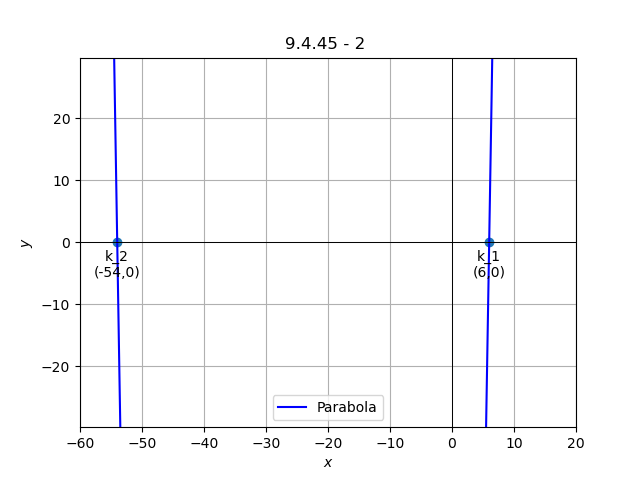
\includegraphics[width=0.5\columnwidth]{figs/graph1_2.png}
    \caption*{}
    \label{fig:placeholder}
\end{figure}


\end{document}


